\newcommand{\NWtarget}[2]{\hypertarget{#1}{#2}}
\newcommand{\NWlink}[2]{\hyperlink{#1}{#2}}
\newcommand{\NWtxtMacroDefBy}{Fragment defined by}
\newcommand{\NWtxtMacroRefIn}{Fragment referenced in}
\newcommand{\NWtxtMacroNoRef}{Fragment never referenced}
\newcommand{\NWtxtDefBy}{Defined by}
\newcommand{\NWtxtRefIn}{Referenced in}
\newcommand{\NWtxtNoRef}{Not referenced}
\newcommand{\NWtxtFileDefBy}{File defined by}
\newcommand{\NWtxtIdentDefinedIn}{defined in}
\newcommand{\NWtxtIdentUsedIn}{used in}
\newcommand{\NWtxtIdentUsers}{Users:}
\newcommand{\NWtxtIdentsNotUsed}{never used}
\newcommand{\NWtxtIdentsUsed}{Uses:}
\newcommand{\NWsep}{${\diamond}$}
\newcommand{\NWnotglobal}{(not defined globally)}
\newcommand{\NWuseHyperlinks}{}
\documentclass[a4paper, 11pt]{article}
\usepackage{fullpage} % for 1.5 cm margins
\renewcommand{\familydefault}{\sfdefault} % so it doesn't look like LaTeX
\usepackage{helvet}
\usepackage{graphicx}
\graphicspath{ {imgs/} }
\usepackage{float} % so the figures stay with the text

\usepackage{abstract}
\renewcommand{\abstractname}{Overview}
\raggedright

\usepackage{parskip}

\usepackage{hyperref}
\hypersetup{
    colorlinks=true,
    linkcolor=blue,
    filecolor=magenta,      
    urlcolor=cyan,
}

\usepackage{listings}
\usepackage{color}
\lstset{language=C++,
        basicstyle=\ttfamily,
        keywordstyle=\color{blue}\ttfamily,
        stringstyle=\color{red}\ttfamily,
        commentstyle=\color{green}\ttfamily,
        morecomment=[l][\color{magenta}]{\#}
}

\title{Promethean Temperature Sensor}
\author{Joe Collins}

\begin{document}
\maketitle
%%%%%%%%%%%%%%%%%%%%%%%%%%%%%%%%%%%%%%%%%%%%%%%%%%%%%%%%%%%%
\tableofcontents
\clearpage

%%%%%%%%%%%%%%%%%%%%%%%%%%%%%%%%%%%%%%%%%%%%%%%%%%%%%%%%%%%%
\section{Objective}

A temperature sensor that can be scraped/polled using \href{https://prometheus.io/}{Prometheus}.

Prometheus is excellent for monitoring server metrics,
so it makes sense to use it to monitor other metrics such as temperature and humidity.
There doesn't appear to be anything available off the shelf.
There are temperature monitors but some effort would be required to get 
them to integrate with Prometheus.
So we might as well build a bespoke temperature sensor
that can be scraped/polled directly by Prometheus.

\begin{figure}[H]
  \centering
  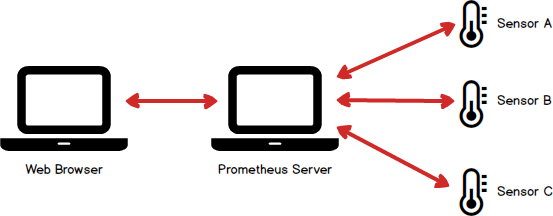
\includegraphics[width=0.75\textwidth]{prometheus.png}
  \caption{Prometheus scraping sensors}
\end{figure}

With Prometheus scraping the temperature sensors,
a web browser can be used to few graphs of the scraped data.

%%%%%%%%%%%%%%%%%%%%%%%%%%%%%%%%%%%%%%%%%%%%%%%%%%%%%%%%%%%%
\section{Components}

Each sensor is an Arduino microcontroller with a temperature sensore attached,
total cost around \pounds 40.

\begin{tabular}{ll}
  \textbf{Component} & \textbf{Cost} \\ 
  \hline
  Arduino Uno Rev3, ATmega328P, CH340G Compatible Board & \pounds 5.79 \\
  UK 9V AC/DC Power Supply Adapter Plug for Arduino Uno & \pounds 7.95 \\
  Ethernet Shield LAN W5100 for Arduino Uno             & \pounds 7.75 \\
  DHT22 AM2302 Digital Temperature and Humidity Sensor  & \pounds 6.90 \\
  0.25 Watt Metal Film Resistor 10k Ohm                 & \pounds 0.99 \\
  Uno Ethernet Shield Case                              & \pounds 10.36 \\
  \hline
  Total cost in November 2020                   & \textbf{\pounds 39.74}  \\
\end{tabular}

\begin{figure}[H]
  \centering
  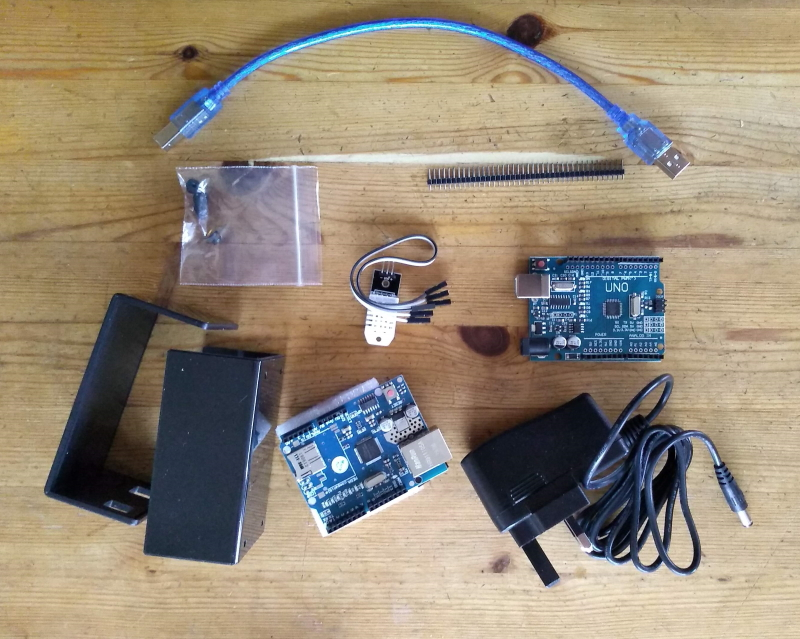
\includegraphics[width=0.75\textwidth]{components.jpg}
  \caption{Components}
\end{figure}

%%%%%%%%%%%%%%%%%%%%%%%%%%%%%%%%%%%%%%%%%%%%%%%%%%%%%%%%%%%%
\section{Wiring the Sensor}
\label{sec:wiring}

The sensor is a DHT22 AM2302 capacitive humidity sensing digital temperature and humidity module.
It is has a calibrated digital signal output of the temperature and humidity sensors.
Other sensors are available such as the cheaper DHT11,
but supposedly it is less sensitive and less durable.
Whilst sensitivity is not important
durability probably is.

The sensor is wired with a 10k Ohm pull up resistor.
This ensures that the signal wire has a small but consistent current,
so it is less susceptible to electrical interference.
In theory you can also set the pin mode with \verb|pinMode("pin", INPUT_PULLUP);|
to use a built in pull up resistor.

The sensor works without the pull up resistor but is probably less accurate
(though I haven't tested it).

\begin{figure}[H]
  \centering
  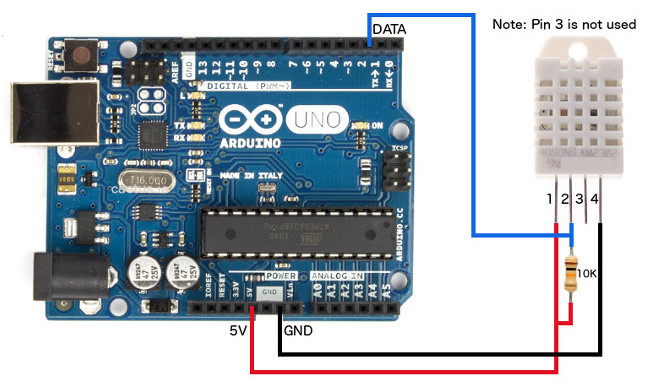
\includegraphics[width=0.75\textwidth]{wiring-dht22.jpg}
  \caption{Wiring diagram with pull up resistor}
\end{figure}

Since the Arduino has an ethernet shield,
practically the wiring looks like this with
insulation around the connectors in case they get moved.

\begin{figure}[H]
  \centering
  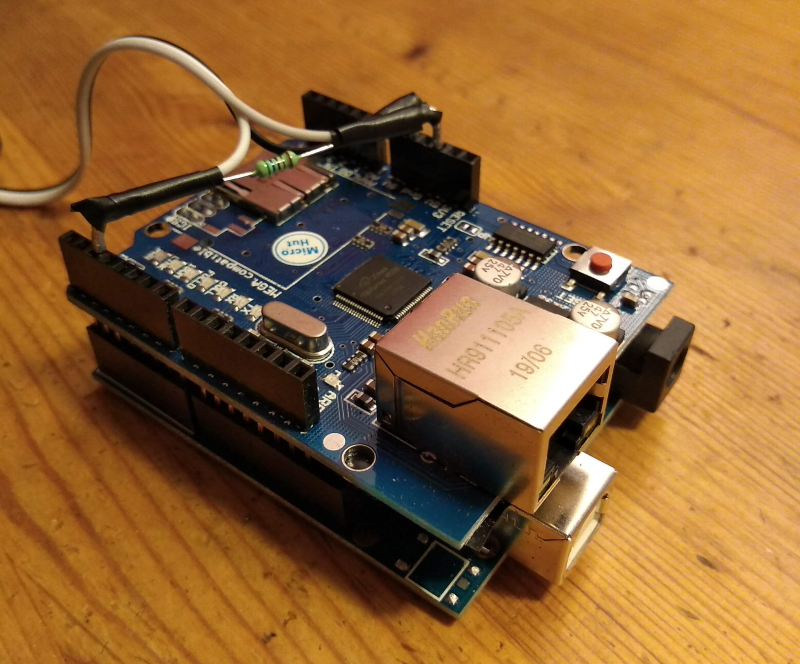
\includegraphics[width=0.75\textwidth]{wiring-with-ethernet.jpg}
  \caption{Wiring with insulation}
\end{figure}

%%%%%%%%%%%%%%%%%%%%%%%%%%%%%%%%%%%%%%%%%%%%%%%%%%%%%%%%%%%%
\section{Programming}

Tooling: 

\begin{itemize}
  \item VSCode \\
  \url{https://code.visualstudio.com/}
  \item PlatformIO \\
  \url{https://marketplace.visualstudio.com/items?itemName=platformio.platformio-ide}
\end{itemize}

The Arduino libraries will need to be installed like this:

\begin{verbatim}
pio lib install "lasselukkari/aWOT"
\end{verbatim}

%%%%%%%%%%%%%%%%%%%%%%%%%%%%%%%%%%%%%%%%%%%%%%%%%%%%%%%%%%%%
\subsection{An Arduino Program}

All Arduino programs have the same format with \verb|setup()| and \verb|loop()| functions.
The \verb|loop()| runs continuously and the \verb|setup()| is run
when the Arduino is turned on
or
when the reset button (red button near the USB socket) is pressed.

\begin{flushleft} \small
\begin{minipage}{\linewidth}\label{scrap1}\raggedright\small
\NWtarget{nuweb5}{}\verb@"../src/main.cpp"@\nobreak\ {\footnotesize{5}}$\equiv$
\vspace{-1ex}
\begin{list}{}{\setlength{\leftmargin}{1em}} \item
\mbox{}\lstinline@#include <Arduino.h>@\\
\mbox{}\lstinline@@$\langle\,${\itshape libraries}\ {\footnotesize \NWlink{nuweb6a}{6a}},\ ...\,$\rangle\,$\verb@@\\
\mbox{}\lstinline@/*** Configuration ***/@\\
\mbox{}\lstinline@@$\langle\,${\itshape configuration}\ {\footnotesize \NWlink{nuweb6b}{6b}},\ ...\,$\rangle\,$\verb@@\\
\mbox{}\lstinline@/*** Functions ***/@\\
\mbox{}\lstinline@@$\langle\,${\itshape functions}\ {\footnotesize \NWlink{nuweb6d}{6d}},\ ...\,$\rangle\,$\verb@@\\
\mbox{}\lstinline@/*** Setup ***/@\\
\mbox{}\lstinline@void setup() @\\
\mbox{}\lstinline@{@\\
\mbox{}\lstinline@  Serial.begin(9600);@\\
\mbox{}\lstinline@  while (!Serial){;}@\\
\mbox{}\lstinline@  @$\langle\,${\itshape setup}\ {\footnotesize \NWlink{nuweb6c}{6c}},\ ...\,$\rangle\,$\verb@@\\
\mbox{}\lstinline@}@\\
\mbox{}\lstinline@/*** Loop ***/@\\
\mbox{}\lstinline@void loop() @\\
\mbox{}\lstinline@{@\\
\mbox{}\lstinline@  @$\langle\,${\itshape loop}\ {\footnotesize \NWlink{nuweb9b}{9b}}\,$\rangle\,$\verb@@\\
\mbox{}\lstinline@}@\\
\mbox{}{\NWsep}
\end{list}
\vspace{-1ex}
\end{minipage}
\end{flushleft}

Since we're using PlatformIO we need the Arduino header (\verb|<Arduino.h>|).
For normal Arduino programs it is not required.

It's useful to be able to connect to the Arduino over the USB cable,
so the \verb|setup()| opens serial for output to monitor and waits for the port to open.
Waiting for the serial port to connect is only needed for native USB ports.

%%%%%%%%%%%%%%%%%%%%%%%%%%%%%%%%%%%%%%%%%%%%%%%%%%%%%%%%%%%%
\subsection{Sensor}

To interact with the DHT22 sensor we need specific drivers (\verb|<DHT.h>|),
which rely on the Adafruit Unified Sensor Driver (\verb|<Adafruit_Sensor.h>|),
The Adafruit Unified Sensor Driver is an abstraction layer
which makes creating reliable drivers is easier. 

The Serial Peripheral Interface (\verb|<SPI.h>|) is a synchronous serial data protocol
used by microcontrollers for communicating with peripheral devices quickly over short distances.

\begin{flushleft} \small
\begin{minipage}{\linewidth}\label{scrap2}\raggedright\small
\NWtarget{nuweb6a}{}$\langle\,${\itshape libraries}\nobreak\ {\footnotesize{6a}}$\,\rangle\equiv$
\vspace{-1ex}
\begin{list}{}{\setlength{\leftmargin}{1em}} \item
\mbox{}\lstinline@#include <Adafruit_Sensor.h>@\\
\mbox{}\lstinline@#include <DHT.h>@\\
\mbox{}\lstinline@#include <SPI.h>@\\
\mbox{}{\NWsep}
\end{list}
\vspace{-1ex}
\vspace{-1ex}
\footnotesize
\begin{list}{}{\setlength{\itemsep}{-\parsep}\setlength{\itemindent}{-\leftmargin}}
\item \NWtxtMacroDefBy\ \NWlink{nuweb6a}{6a}, \NWlink{nuweb7b}{7b}.
\item \NWtxtMacroRefIn\ \NWlink{nuweb5}{5}.
\end{list}
\end{minipage}
\end{flushleft}

The sensor communicates using pin 2 (see \hyperref[sec:wiring]{wiring})
and
the sensor type needs to be set.
The temperature and humidity
are stored in global variables
since they'll be used by pretty much every part of the program.

\begin{flushleft} \small
\begin{minipage}{\linewidth}\label{scrap3}\raggedright\small
\NWtarget{nuweb6b}{}$\langle\,${\itshape configuration}\nobreak\ {\footnotesize{6b}}$\,\rangle\equiv$
\vspace{-1ex}
\begin{list}{}{\setlength{\leftmargin}{1em}} \item
\mbox{}\lstinline@#define DHTPIN 2@\\
\mbox{}\lstinline@#define DHTTYPE DHT22@\\
\mbox{}\lstinline@DHT dht = DHT(DHTPIN, DHTTYPE);@\\
\mbox{}\lstinline@float temperature = 0;@\\
\mbox{}\lstinline@float humidity = 0;@\\
\mbox{}{\NWsep}
\end{list}
\vspace{-1ex}
\vspace{-1ex}
\footnotesize
\begin{list}{}{\setlength{\itemsep}{-\parsep}\setlength{\itemindent}{-\leftmargin}}
\item \NWtxtMacroDefBy\ \NWlink{nuweb6b}{6b}, \NWlink{nuweb7c}{7c}.
\item \NWtxtMacroRefIn\ \NWlink{nuweb5}{5}.
\end{list}
\end{minipage}
\end{flushleft}

The sensor needs to \verb|begin()|.
Formerly this method was used to pass in parameters relating the the speed of the Arduino.
Now the sensor automatically adapts
but \verb|begin()| is still needed.

\begin{flushleft} \small
\begin{minipage}{\linewidth}\label{scrap4}\raggedright\small
\NWtarget{nuweb6c}{}$\langle\,${\itshape setup}\nobreak\ {\footnotesize{6c}}$\,\rangle\equiv$
\vspace{-1ex}
\begin{list}{}{\setlength{\leftmargin}{1em}} \item
\mbox{}\lstinline@Serial.println("Set up sensor");@\\
\mbox{}\lstinline@dht.begin();@\\
\mbox{}{\NWsep}
\end{list}
\vspace{-1ex}
\vspace{-1ex}
\footnotesize
\begin{list}{}{\setlength{\itemsep}{-\parsep}\setlength{\itemindent}{-\leftmargin}}
\item \NWtxtMacroDefBy\ \NWlink{nuweb6c}{6c}, \NWlink{nuweb8a}{8a}\NWlink{nuweb8b}{b}.
\item \NWtxtMacroRefIn\ \NWlink{nuweb5}{5}.
\end{list}
\end{minipage}
\end{flushleft}

Set the values of humidity (as a percentage)
and the temperature (as Celsius) as globals.
This is largely so I don't have to bother passing the values around.
In the event that nothing comes back from the sensor,
the values of \verb|humidity| and \verb|temperature|
won't get reset.
So if the DHT22 sensor fails in use
the device will carry on reporting old
(but plausible) values
until the Arduino is reset.

\begin{flushleft} \small
\begin{minipage}{\linewidth}\label{scrap5}\raggedright\small
\NWtarget{nuweb6d}{}$\langle\,${\itshape functions}\nobreak\ {\footnotesize{6d}}$\,\rangle\equiv$
\vspace{-1ex}
\begin{list}{}{\setlength{\leftmargin}{1em}} \item
\mbox{}\lstinline@void readSensor()@\\
\mbox{}\lstinline@{@\\
\mbox{}\lstinline@  humidity = dht.readHumidity();@\\
\mbox{}\lstinline@  temperature = dht.readTemperature();@\\
\mbox{}\lstinline@  if (isnan(humidity) || isnan(temperature)) @\\
\mbox{}\lstinline@  {@\\
\mbox{}\lstinline@    Serial.println("Failed to read from sensor");@\\
\mbox{}\lstinline@    return;@\\
\mbox{}\lstinline@  }@\\
\mbox{}\lstinline@}@\\
\mbox{}{\NWsep}
\end{list}
\vspace{-1ex}
\vspace{-1ex}
\footnotesize
\begin{list}{}{\setlength{\itemsep}{-\parsep}\setlength{\itemindent}{-\leftmargin}}
\item \NWtxtMacroDefBy\ \NWlink{nuweb6d}{6d}, \NWlink{nuweb7a}{7a}, \NWlink{nuweb8c}{8c}, \NWlink{nuweb9a}{9a}.
\item \NWtxtMacroRefIn\ \NWlink{nuweb5}{5}.
\end{list}
\end{minipage}
\end{flushleft}

In use there is no need to write out to the serial monitor,
since the USB cable will not be attached.
However, during development it is handy to be able to see what is going on.

\begin{flushleft} \small
\begin{minipage}{\linewidth}\label{scrap6}\raggedright\small
\NWtarget{nuweb7a}{}$\langle\,${\itshape functions}\nobreak\ {\footnotesize{7a}}$\,\rangle\equiv$
\vspace{-1ex}
\begin{list}{}{\setlength{\leftmargin}{1em}} \item
\mbox{}\lstinline@void serialPrintReadings()@\\
\mbox{}\lstinline@{@\\
\mbox{}\lstinline@  Serial.print("Humidity: ");@\\
\mbox{}\lstinline@  Serial.print(humidity);@\\
\mbox{}\lstinline@  Serial.print(" % | ");@\\
\mbox{}\lstinline@  Serial.print("Temperature: ");@\\
\mbox{}\lstinline@  Serial.print(temperature);@\\
\mbox{}\lstinline@  Serial.println(" C");@\\
\mbox{}\lstinline@}@\\
\mbox{}{\NWsep}
\end{list}
\vspace{-1ex}
\vspace{-1ex}
\footnotesize
\begin{list}{}{\setlength{\itemsep}{-\parsep}\setlength{\itemindent}{-\leftmargin}}
\item \NWtxtMacroDefBy\ \NWlink{nuweb6d}{6d}, \NWlink{nuweb7a}{7a}, \NWlink{nuweb8c}{8c}, \NWlink{nuweb9a}{9a}.
\item \NWtxtMacroRefIn\ \NWlink{nuweb5}{5}.
\end{list}
\end{minipage}
\end{flushleft}

%%%%%%%%%%%%%%%%%%%%%%%%%%%%%%%%%%%%%%%%%%%%%%%%%%%%%%%%%%%%
\subsection{Ethernet Client}

The goal is to provide an HTTP end point for Prometheus to scrape data from.
This is possible using just \verb|<Ethernet.h>|
(the library for the ethernet)
but this approach only allows for one web page and no routing.
Typically Prometheus expects the metrics to be on a route at \verb|/metrics|.
Also having routing would give the possibility of having a more friendly webpage showing the readings.

The Arduino web server library \href{https://github.com/lasselukkari/awot}{Arduino web server library}.
The package downloaded by PlatformIO is marked
\verb|lasselukkari/aWOT@0.0.0-alpha+sha.bf07e6371c|
which is curious since the rest of the meta data indicates that it is version 3.0.2
(the current latest version).

\begin{flushleft} \small
\begin{minipage}{\linewidth}\label{scrap7}\raggedright\small
\NWtarget{nuweb7b}{}$\langle\,${\itshape libraries}\nobreak\ {\footnotesize{7b}}$\,\rangle\equiv$
\vspace{-1ex}
\begin{list}{}{\setlength{\leftmargin}{1em}} \item
\mbox{}\lstinline@#include <Ethernet.h>@\\
\mbox{}\lstinline@#include <aWOT.h>@\\
\mbox{}{\NWsep}
\end{list}
\vspace{-1ex}
\vspace{-1ex}
\footnotesize
\begin{list}{}{\setlength{\itemsep}{-\parsep}\setlength{\itemindent}{-\leftmargin}}
\item \NWtxtMacroDefBy\ \NWlink{nuweb6a}{6a}, \NWlink{nuweb7b}{7b}.
\item \NWtxtMacroRefIn\ \NWlink{nuweb5}{5}.
\end{list}
\end{minipage}
\end{flushleft}

The MAC address and IP address for the device
are provided as global values.
This isn't strictly necessary since they are only used once in the \verb|setup()|
but this is the pattern followed by most examples I found so I did the same.
However it is useful for the \verb|server| and the \verb|app| to be available
as global variables since the \verb|loop()| makes repeated use of them.
The MAC address might be written on the ethernet shield,
but if it isn't you can just make one up (or use an on-line generator).
Either way the MAC address like the IP address
should be unique to the device you are making.

\begin{flushleft} \small
\begin{minipage}{\linewidth}\label{scrap8}\raggedright\small
\NWtarget{nuweb7c}{}$\langle\,${\itshape configuration}\nobreak\ {\footnotesize{7c}}$\,\rangle\equiv$
\vspace{-1ex}
\begin{list}{}{\setlength{\leftmargin}{1em}} \item
\mbox{}\lstinline@byte mac[] = {@\\
\mbox{}\lstinline@  0xF6, 0x54, 0xA8, 0x28, 0xE5, 0xD0@\\
\mbox{}\lstinline@};@\\
\mbox{}\lstinline@IPAddress ip(10, 0, 21, 212);@\\
\mbox{}\lstinline@EthernetServer server(80);@\\
\mbox{}\lstinline@Application app;@\\
\mbox{}{\NWsep}
\end{list}
\vspace{-1ex}
\vspace{-1ex}
\footnotesize
\begin{list}{}{\setlength{\itemsep}{-\parsep}\setlength{\itemindent}{-\leftmargin}}
\item \NWtxtMacroDefBy\ \NWlink{nuweb6b}{6b}, \NWlink{nuweb7c}{7c}.
\item \NWtxtMacroRefIn\ \NWlink{nuweb5}{5}.
\end{list}
\end{minipage}
\end{flushleft}

The MAC address and IP address are then used in the \verb|setup()|
to initialize the ethernet shield
and confirm that it is present and working.

\begin{flushleft} \small
\begin{minipage}{\linewidth}\label{scrap9}\raggedright\small
\NWtarget{nuweb8a}{}$\langle\,${\itshape setup}\nobreak\ {\footnotesize{8a}}$\,\rangle\equiv$
\vspace{-1ex}
\begin{list}{}{\setlength{\leftmargin}{1em}} \item
\mbox{}\lstinline@Ethernet.begin(mac, ip);@\\
\mbox{}\lstinline@if (Ethernet.hardwareStatus() == EthernetNoHardware) @\\
\mbox{}\lstinline@{@\\
\mbox{}\lstinline@  Serial.println("Ethernet shield was not found.");@\\
\mbox{}\lstinline@  while (true) @\\
\mbox{}\lstinline@  {@\\
\mbox{}\lstinline@    delay(1); // Do nothing since there is no point in proceeding.@\\
\mbox{}\lstinline@  }@\\
\mbox{}\lstinline@}@\\
\mbox{}\lstinline@if (Ethernet.linkStatus() == LinkOFF) {@\\
\mbox{}\lstinline@  Serial.println("Ethernet cable is not connected.");@\\
\mbox{}\lstinline@}@\\
\mbox{}{\NWsep}
\end{list}
\vspace{-1ex}
\vspace{-1ex}
\footnotesize
\begin{list}{}{\setlength{\itemsep}{-\parsep}\setlength{\itemindent}{-\leftmargin}}
\item \NWtxtMacroDefBy\ \NWlink{nuweb6c}{6c}, \NWlink{nuweb8a}{8a}\NWlink{nuweb8b}{b}.
\item \NWtxtMacroRefIn\ \NWlink{nuweb5}{5}.
\end{list}
\end{minipage}
\end{flushleft}

Two routes are provided,
one to `/' for a web page and one to `/metrics' for the Prometheus metrics.

\begin{flushleft} \small
\begin{minipage}{\linewidth}\label{scrap10}\raggedright\small
\NWtarget{nuweb8b}{}$\langle\,${\itshape setup}\nobreak\ {\footnotesize{8b}}$\,\rangle\equiv$
\vspace{-1ex}
\begin{list}{}{\setlength{\leftmargin}{1em}} \item
\mbox{}\lstinline@app.get("/", &indexCmd);@\\
\mbox{}\lstinline@app.get("/metrics", &metricsCmd);@\\
\mbox{}{\NWsep}
\end{list}
\vspace{-1ex}
\vspace{-1ex}
\footnotesize
\begin{list}{}{\setlength{\itemsep}{-\parsep}\setlength{\itemindent}{-\leftmargin}}
\item \NWtxtMacroDefBy\ \NWlink{nuweb6c}{6c}, \NWlink{nuweb8a}{8a}\NWlink{nuweb8b}{b}.
\item \NWtxtMacroRefIn\ \NWlink{nuweb5}{5}.
\end{list}
\end{minipage}
\end{flushleft}

The web page is as simple as can be but refreshes at regular intervals to show the temperature.

\begin{flushleft} \small
\begin{minipage}{\linewidth}\label{scrap11}\raggedright\small
\NWtarget{nuweb8c}{}$\langle\,${\itshape functions}\nobreak\ {\footnotesize{8c}}$\,\rangle\equiv$
\vspace{-1ex}
\begin{list}{}{\setlength{\leftmargin}{1em}} \item
\mbox{}\lstinline@void indexCmd(Request &req, Response &res)@\\
\mbox{}\lstinline@{@\\
\mbox{}\lstinline@  Serial.println("Request for index");@\\
\mbox{}\lstinline@  res.set("Content-Type", "text/html");@\\
\mbox{}\lstinline@  res.println("<html>");@\\
\mbox{}\lstinline@  res.println("<head>");@\\
\mbox{}\lstinline@  res.println("  <meta http-equiv=\"refresh\" content=\"5\">");@\\
\mbox{}\lstinline@  res.println("</head>");@\\
\mbox{}\lstinline@  res.println("<body>");@\\
\mbox{}\lstinline@  res.println("  <H1>Temp: " + String(temperature) + "</p>");@\\
\mbox{}\lstinline@  res.println("</body>");@\\
\mbox{}\lstinline@  res.println("</html>");@\\
\mbox{}\lstinline@}@\\
\mbox{}{\NWsep}
\end{list}
\vspace{-1ex}
\vspace{-1ex}
\footnotesize
\begin{list}{}{\setlength{\itemsep}{-\parsep}\setlength{\itemindent}{-\leftmargin}}
\item \NWtxtMacroDefBy\ \NWlink{nuweb6d}{6d}, \NWlink{nuweb7a}{7a}, \NWlink{nuweb8c}{8c}, \NWlink{nuweb9a}{9a}.
\item \NWtxtMacroRefIn\ \NWlink{nuweb5}{5}.
\end{list}
\end{minipage}
\end{flushleft}

Prometheus has a particular style for showing metrics ready for scraping.
In this case both humidity and temperature are gauges,
values that vary.
For interest the alternative Prometheus metric type is a counter,
for values that increase.

\begin{flushleft} \small
\begin{minipage}{\linewidth}\label{scrap12}\raggedright\small
\NWtarget{nuweb9a}{}$\langle\,${\itshape functions}\nobreak\ {\footnotesize{9a}}$\,\rangle\equiv$
\vspace{-1ex}
\begin{list}{}{\setlength{\leftmargin}{1em}} \item
\mbox{}\lstinline@void metricsCmd(Request &req, Response &res)@\\
\mbox{}\lstinline@{@\\
\mbox{}\lstinline@  Serial.println("Request for metrics");@\\
\mbox{}\lstinline@  res.set("Content-Type", "text/plain");@\\
\mbox{}\lstinline@  res.print("# HELP temperature is the last temperature reading in degrees celsius\n");@\\
\mbox{}\lstinline@  res.print("# TYPE temp gauge\n");@\\
\mbox{}\lstinline@  res.print("temperature " + String(temperature) + "\n");@\\
\mbox{}\lstinline@  res.print("# HELP humidity is the last relative humidity reading as a percentage\n");@\\
\mbox{}\lstinline@  res.print("# TYPE humidity gauge\n");@\\
\mbox{}\lstinline@  res.print("humidity " + String(humidity) + "\n");@\\
\mbox{}\lstinline@}@\\
\mbox{}{\NWsep}
\end{list}
\vspace{-1ex}
\vspace{-1ex}
\footnotesize
\begin{list}{}{\setlength{\itemsep}{-\parsep}\setlength{\itemindent}{-\leftmargin}}
\item \NWtxtMacroDefBy\ \NWlink{nuweb6d}{6d}, \NWlink{nuweb7a}{7a}, \NWlink{nuweb8c}{8c}, \NWlink{nuweb9a}{9a}.
\item \NWtxtMacroRefIn\ \NWlink{nuweb5}{5}.
\end{list}
\end{minipage}
\end{flushleft}

Most of the time the Arduino is running through this loop.
It takes about 250 milliseconds to read from the sensor.
The 2 second delay is to prevent reading from the sensor faster than it can respond.
This does mean that a request from Prometheus for data might be delayed by up to 2 seconds
before the web server can respond.

\begin{flushleft} \small
\begin{minipage}{\linewidth}\label{scrap13}\raggedright\small
\NWtarget{nuweb9b}{}$\langle\,${\itshape loop}\nobreak\ {\footnotesize{9b}}$\,\rangle\equiv$
\vspace{-1ex}
\begin{list}{}{\setlength{\leftmargin}{1em}} \item
\mbox{}\lstinline@  delay(2000);@\\
\mbox{}\lstinline@  readSensor();@\\
\mbox{}\lstinline@  serialPrintReadings();@\\
\mbox{}\lstinline@  EthernetClient client = server.available();@\\
\mbox{}\lstinline@  if (client.connected()) {@\\
\mbox{}\lstinline@    app.process(&client);@\\
\mbox{}\lstinline@    client.stop();@\\
\mbox{}\lstinline@  }@\\
\mbox{}{\NWsep}
\end{list}
\vspace{-1ex}
\vspace{-1ex}
\footnotesize
\begin{list}{}{\setlength{\itemsep}{-\parsep}\setlength{\itemindent}{-\leftmargin}}
\item \NWtxtMacroRefIn\ \NWlink{nuweb5}{5}.
\end{list}
\end{minipage}
\end{flushleft}

%%%%%%%%%%%%%%%%%%%%%%%%%%%%%%%%%%%%%%%%%%%%%%%%%%%%%%%%%%%%
\subsection{Build and Upload}

The PlatformIO extension with VSCode includes
commands to 
\verb|PlatformIO: Build|
and
\verb|PlatformIO: Upload|.
Initially the upload did not work so I installed CH340 drivers
on the advice of this reference \url{https://nagesh-uluvar.blogspot.com/2016/12/arduino-not-getting-detected-usb20.html}.
The short answer is to install these drivers \url{https://sites.google.com/site/nageshuluvar/home/DRIVER1_CH340.zip?attredirects=0&d=1}.
There are versions at \url{https://sparks.gogo.co.nz/ch340.html} for the Mac as well.

Additionally the upload was sometimes unreliable.
It appears that PlatformIO attempts to read back the uploaded file.
The read back doesn't always work,
but more often that not the file had been successfully uploaded to the Arduino.

%%%%%%%%%%%%%%%%%%%%%%%%%%%%%%%%%%%%%%%%%%%%%%%%%%%%%%%%%%%%
\subsection{Testing}

Once the files have been uploaded to the Arduino,
it should restart and the serial monitor should show something like this.

\begin{verbatim}
  --- Quit: Ctrl+C | Menu: Ctrl+T | Help: Ctrl+T followed by Ctrl+H ---
  Webserver set up
  Sensor set up
  Humidity: 55.90 % | Temperature: 22.10 C
  Humidity: 56.30 % | Temperature: 22.20 C
\end{verbatim}

To test the Prometheus end point you can use an ethernet patch cable to connect to it directly
(rather than via a router).

\begin{itemize}
  \item Assign a manual IP address to the laptop's ethernet connection say 10.0.21.1.
  \item Subnet mask 255.255.255.0.
  \item Assign a manual IP address to the Arduino's ethernet, say 10.0.21.212.
  \item Subnet mask 255.255.255.0.
  \item Leave the default Gateway empty.
  \item Use an ethernet patch cable to link the two (since 100BaseT onwards it doesn't have to be a special cross over cable).
  \item You should then be able to get your Arduino site up on \url{http://192.168.0.2} from the laptop.
\end{itemize}
  
This is the endpoint at \url{http://10.0.21.212/metrics} which should show something like this.
  
\begin{verbatim}
  > curl 10.0.21.212
  # HELP temperature is the last temperature reading in degrees celsius
  # TYPE temp gauge
  temperature 23.30
  # HELP humidity is the last relative humidity reading as a percentage
  # TYPE humidity gauge
  humidity 47.60
\end{verbatim}

The Prometheus server is available as a docker image,
so you can run it up with \verb|docker-compose up|.
The Prometheus interface should be available at \url{http://localhost:9090}
and should be able to provide a graph like this.

\begin{figure}[H]
  \centering
  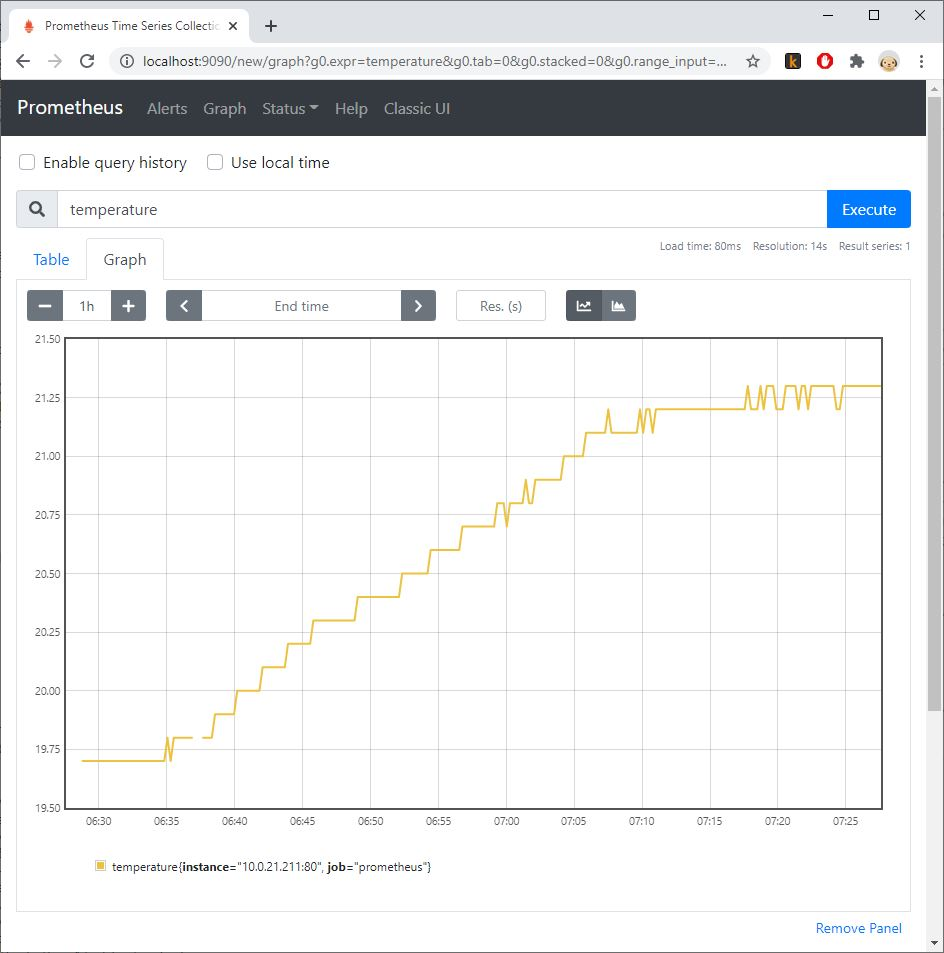
\includegraphics[width=0.75\textwidth]{graph.jpg}
  \caption{Temperature graph}
\end{figure}
  
%%%%%%%%%%%%%%%%%%%%%%%%%%%%%%%%%%%%%%%%%%%%%%%%%%%%%%%%%%%%
\section{Packaging}

The Arduino does put out a bit of heat,
so it doesn't make sense to mount the temperature
sensor directly on the case.
Hence it is mounted on a milk bottle top.
The cable tie is 2.5 mm wide so the holes are 2.5 mm in diameter.
The hold for the wires has a 4mm diameter.

\begin{figure}[H]
  \centering
  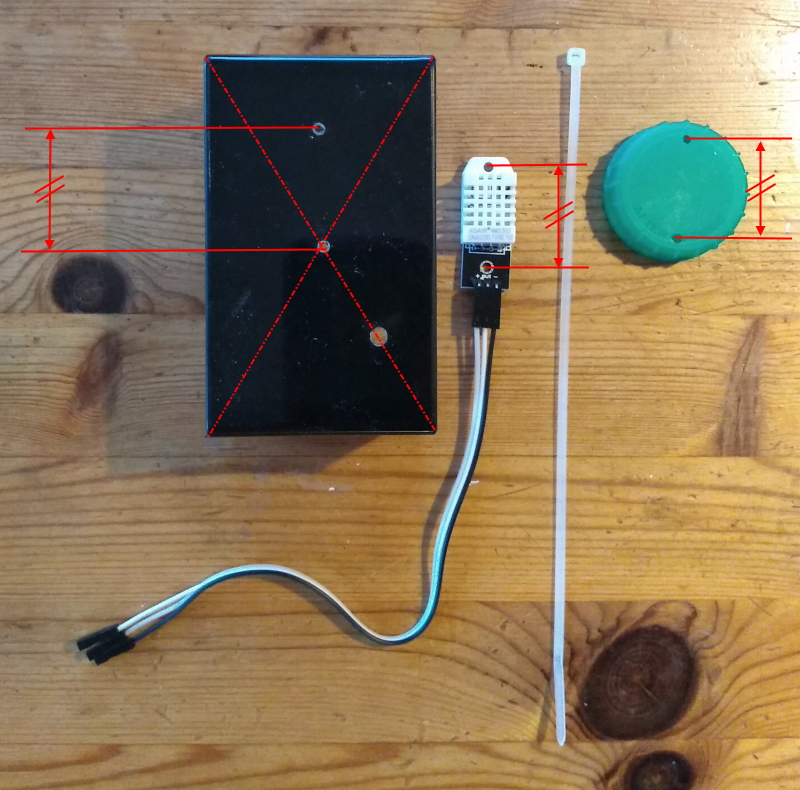
\includegraphics[width=0.75\textwidth]{sensor-mount.jpg}
  \caption{Components for mounting the sensor}
\end{figure}

\begin{figure}[H]
  \centering
  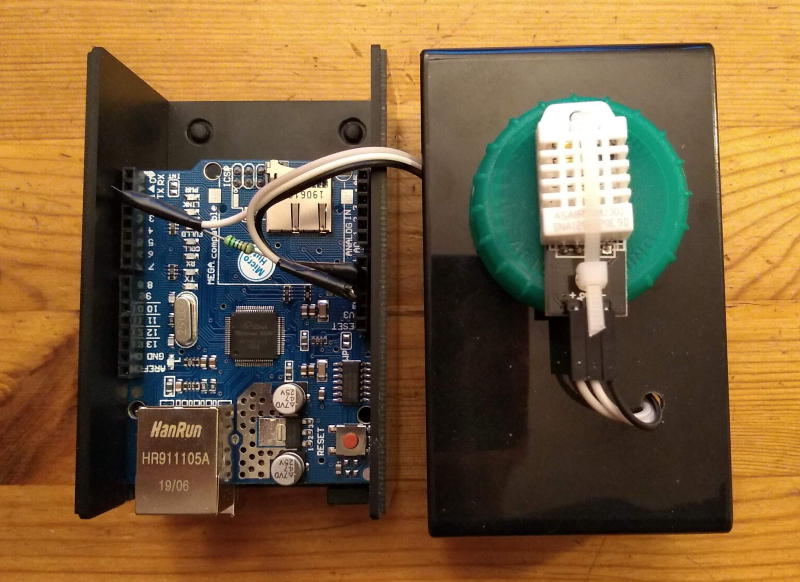
\includegraphics[width=0.75\textwidth]{packaging.jpg}
  \caption{Mounted sensor and wiring}
\end{figure}

\end{document}